\documentclass[11pt,a4paper,]{article}
\usepackage{lmodern}

\usepackage{amssymb,amsmath}
\usepackage{ifxetex,ifluatex}
\usepackage{fixltx2e} % provides \textsubscript
\ifnum 0\ifxetex 1\fi\ifluatex 1\fi=0 % if pdftex
  \usepackage[T1]{fontenc}
  \usepackage[utf8]{inputenc}
\else % if luatex or xelatex
  \usepackage{unicode-math}
  \defaultfontfeatures{Ligatures=TeX,Scale=MatchLowercase}
\fi
% use upquote if available, for straight quotes in verbatim environments
\IfFileExists{upquote.sty}{\usepackage{upquote}}{}
% use microtype if available
\IfFileExists{microtype.sty}{%
\usepackage[]{microtype}
\UseMicrotypeSet[protrusion]{basicmath} % disable protrusion for tt fonts
}{}
\PassOptionsToPackage{hyphens}{url} % url is loaded by hyperref
\usepackage[unicode=true]{hyperref}
\hypersetup{
            pdftitle={Report on Happiness up to 2022},
            pdfborder={0 0 0},
            breaklinks=true}
\urlstyle{same}  % don't use monospace font for urls
\usepackage{geometry}
\geometry{a4paper, centering, text={16cm,25cm}}
\usepackage[style=authoryear-comp,]{biblatex}
\addbibresource{references.bib}
\usepackage{longtable,booktabs}
% Fix footnotes in tables (requires footnote package)
\IfFileExists{footnote.sty}{\usepackage{footnote}\makesavenoteenv{long table}}{}
\usepackage{graphicx,grffile}
\makeatletter
\def\maxwidth{\ifdim\Gin@nat@width>\linewidth\linewidth\else\Gin@nat@width\fi}
\def\maxheight{\ifdim\Gin@nat@height>\textheight\textheight\else\Gin@nat@height\fi}
\makeatother
% Scale images if necessary, so that they will not overflow the page
% margins by default, and it is still possible to overwrite the defaults
% using explicit options in \includegraphics[width, height, ...]{}
\setkeys{Gin}{width=\maxwidth,height=\maxheight,keepaspectratio}
\IfFileExists{parskip.sty}{%
\usepackage{parskip}
}{% else
\setlength{\parindent}{0pt}
\setlength{\parskip}{6pt plus 2pt minus 1pt}
}
\setlength{\emergencystretch}{3em}  % prevent overfull lines
\providecommand{\tightlist}{%
  \setlength{\itemsep}{0pt}\setlength{\parskip}{0pt}}
\setcounter{secnumdepth}{5}

% set default figure placement to htbp
\makeatletter
\def\fps@figure{htbp}
\makeatother


\title{Report on Happiness up to 2022}

%% MONASH STUFF

%% CAPTIONS
\RequirePackage{caption}
\DeclareCaptionStyle{italic}[justification=centering]
 {labelfont={bf},textfont={it},labelsep=colon}
\captionsetup[figure]{style=italic,format=hang,singlelinecheck=true}
\captionsetup[table]{style=italic,format=hang,singlelinecheck=true}


%% FONT
\RequirePackage{bera}
\RequirePackage[charter,expert,sfscaled]{mathdesign}
\RequirePackage{fontawesome}

%% HEADERS AND FOOTERS
\RequirePackage{fancyhdr}
\pagestyle{fancy}
\rfoot{\Large\sffamily\raisebox{-0.1cm}{\textbf{\thepage}}}
\makeatletter
\lhead{\textsf{\expandafter{\@title}}}
\makeatother
\rhead{}
\cfoot{}
\setlength{\headheight}{15pt}
\renewcommand{\headrulewidth}{0.4pt}
\renewcommand{\footrulewidth}{0.4pt}
\fancypagestyle{plain}{%
\fancyhf{} % clear all header and footer fields
\fancyfoot[C]{\sffamily\thepage} % except the center
\renewcommand{\headrulewidth}{0pt}
\renewcommand{\footrulewidth}{0pt}}

%% MATHS
\RequirePackage{bm,amsmath}
\allowdisplaybreaks

%% GRAPHICS
\RequirePackage{graphicx}
\setcounter{topnumber}{2}
\setcounter{bottomnumber}{2}
\setcounter{totalnumber}{4}
\renewcommand{\topfraction}{0.85}
\renewcommand{\bottomfraction}{0.85}
\renewcommand{\textfraction}{0.15}
\renewcommand{\floatpagefraction}{0.8}


%\RequirePackage[section]{placeins}

%% SECTION TITLES


%% SECTION TITLES
\RequirePackage[compact,sf,bf]{titlesec}
\titleformat*{\section}{\Large\sf\bfseries\color[rgb]{0.7,0,0}}
\titleformat*{\subsection}{\large\sf\bfseries\color[rgb]{0.7,0,0}}
\titleformat*{\subsubsection}{\sf\bfseries\color[rgb]{0.7,0,0}}
\titlespacing{\section}{0pt}{2ex}{.5ex}
\titlespacing{\subsection}{0pt}{1.5ex}{0ex}
\titlespacing{\subsubsection}{0pt}{.5ex}{0ex}


%% TITLE PAGE
\def\Date{\number\day}
\def\Month{\ifcase\month\or
 January\or February\or March\or April\or May\or June\or
 July\or August\or September\or October\or November\or December\fi}
\def\Year{\number\year}

%% LINE AND PAGE BREAKING
\sloppy
\clubpenalty = 10000
\widowpenalty = 10000
\brokenpenalty = 10000
\RequirePackage{microtype}

%% PARAGRAPH BREAKS
\setlength{\parskip}{1.4ex}
\setlength{\parindent}{0em}

%% HYPERLINKS
\RequirePackage{xcolor} % Needed for links
\definecolor{darkblue}{rgb}{0,0,.6}
\RequirePackage{url}

\makeatletter
\@ifpackageloaded{hyperref}{}{\RequirePackage{hyperref}}
\makeatother
\hypersetup{
     citecolor=0 0 0,
     breaklinks=true,
     bookmarksopen=true,
     bookmarksnumbered=true,
     linkcolor=darkblue,
     urlcolor=blue,
     citecolor=darkblue,
     colorlinks=true}

\usepackage[showonlyrefs]{mathtools}
\usepackage[no-weekday]{eukdate}

%% BIBLIOGRAPHY

\makeatletter
\@ifpackageloaded{biblatex}{}{\usepackage[style=authoryear-comp, backend=biber, natbib=true]{biblatex}}
\makeatother
\ExecuteBibliographyOptions{bibencoding=utf8,minnames=1,maxnames=3, maxbibnames=99,dashed=false,terseinits=true,giveninits=true,uniquename=false,uniquelist=false,doi=false, isbn=false,url=true,sortcites=false}

\DeclareFieldFormat{url}{\texttt{\url{#1}}}
\DeclareFieldFormat[article]{pages}{#1}
\DeclareFieldFormat[inproceedings]{pages}{\lowercase{pp.}#1}
\DeclareFieldFormat[incollection]{pages}{\lowercase{pp.}#1}
\DeclareFieldFormat[article]{volume}{\mkbibbold{#1}}
\DeclareFieldFormat[article]{number}{\mkbibparens{#1}}
\DeclareFieldFormat[article]{title}{\MakeCapital{#1}}
\DeclareFieldFormat[article]{url}{}
%\DeclareFieldFormat[book]{url}{}
%\DeclareFieldFormat[inbook]{url}{}
%\DeclareFieldFormat[incollection]{url}{}
%\DeclareFieldFormat[inproceedings]{url}{}
\DeclareFieldFormat[inproceedings]{title}{#1}
\DeclareFieldFormat{shorthandwidth}{#1}
%\DeclareFieldFormat{extrayear}{}
% No dot before number of articles
\usepackage{xpatch}
\xpatchbibmacro{volume+number+eid}{\setunit*{\adddot}}{}{}{}
% Remove In: for an article.
\renewbibmacro{in:}{%
  \ifentrytype{article}{}{%
  \printtext{\bibstring{in}\intitlepunct}}}

\AtEveryBibitem{\clearfield{month}}
\AtEveryCitekey{\clearfield{month}}

\makeatletter
\DeclareDelimFormat[cbx@textcite]{nameyeardelim}{\addspace}
\makeatother

\author{\sf{\Large\textbf{Zhixiang Yang}\\\large EBS Honours Student\\[0.5cm]}{\Large\textbf{Yiqi Wang}\\\large Master of BA Student\\[0.5cm]}{\Large\textbf{Xintong You}\\\large Master of BA Student\\[0.5cm]}}

\date{\sf\Date~\Month~\Year}
\makeatletter
\lfoot{\sf Yang, Wang, You: \@date}
\makeatother


%%%% PAGE STYLE FOR FRONT PAGE OF REPORTS

\makeatletter
\def\organization#1{\gdef\@organization{#1}}
\def\telephone#1{\gdef\@telephone{#1}}
\def\email#1{\gdef\@email{#1}}
\makeatother
  \organization{Group 07 ETC5513}

  \def\name{Department of\newline Econometrics \&\newline Business Statistics}

  \telephone{(03) 9905 2478}

  \email{BusEco-Econometrics@monash.edu}

\def\webaddress{\url{http://buseco.monash.edu/ebs/consulting/}}
\def\abn{12 377 614 012}
\def\extraspace{\vspace*{1.6cm}}
\makeatletter
\def\contactdetails{\faicon{phone} & \@telephone \\
                    \faicon{envelope} & \@email}
\makeatother

\usepackage[absolute,overlay]{textpos}
\setlength{\TPHorizModule}{1cm}
\setlength{\TPVertModule}{1cm}

%%%% FRONT PAGE OF REPORTS

\def\reporttype{Report for}

\long\def\front#1#2#3{
\newpage
\begin{textblock}{7}(12.7,28.2)\hfill

\includegraphics[height=0.6cm]{AACSB}~~~

\includegraphics[height=0.6cm]{EQUIS}~~~

\includegraphics[height=0.6cm]{AMBA}
\end{textblock}
\begin{singlespacing}
\thispagestyle{empty}
\vspace*{-1.4cm}
\hspace*{-1.4cm}
\hbox to 16cm{
  \hbox to 6.5cm{\vbox to 14cm{\vbox to 25cm{
    
\includegraphics[width=6cm]{monash2}
    \vfill
    
\includegraphics[width=3.5cm]{MBSportrait}
    \vspace{0.4cm}
    \par
    \parbox{6.3cm}{\raggedright
      \sf\color[rgb]{0.00,0.00,0.70}
      {\large\textbf{\name}}\par
      \vspace{.7cm}
      \tabcolsep=0.12cm\sf\small
      \begin{tabular}{@{}ll@{}}\contactdetails
      \end{tabular}
      \vspace*{0.3cm}\par
      ABN: \abn\par
    }
  }\vss}\hss}
  \hspace*{0.2cm}
  \hbox to 1cm{\vbox to 14cm{\rule{1pt}{26.8cm}\vss}\hss\hfill}
  \hbox to 10cm{\vbox to 14cm{\vbox to 25cm{
      \vspace*{3cm}\sf\raggedright
      \parbox{11cm}{\sf\raggedright\baselineskip=1.2cm
         \fontsize{24.88}{30}\color[rgb]{0.70,0.00,0.00}\sf\textbf{#1}}
      \par
      \vfill
      \large
      \vbox{\parskip=0.8cm #2}\par
      \vspace*{2cm}\par
      \reporttype\\[0.3cm]
      \hbox{#3}%\\[2cm]\
      \vspace*{1cm}
      {\large\sf\textbf{\Date~\Month~\Year}}
   }\vss}
  }}
\end{singlespacing}
\newpage
}

\makeatletter
\def\titlepage{\front{\expandafter{\@title}}{\@author}{\@organization}}
\makeatother

\usepackage{setspace}
\setstretch{1.5}

%% Any special functions or other packages can be loaded here.
\usepackage[normalem]{ulem}
\usepackage{float}

\useunder{\uline}{\ul}{}
\usepackage{float}
\usepackage{booktabs}
\usepackage{longtable}
\usepackage{array}
\usepackage{multirow}
\usepackage{wrapfig}
\usepackage{colortbl}
\usepackage{pdflscape}
\usepackage{tabu}
\usepackage{threeparttable}
\usepackage{threeparttablex}
\usepackage[normalem]{ulem}
\usepackage{makecell}
\usepackage{xcolor}


\begin{document}
\titlepage

\hypertarget{modelling}{%
\section{Modelling}\label{modelling}}

\hypertarget{what-is-the-most-important-variable-to-explain-the-happiness-score-differences-across-different-countries-in-different-years}{%
\subsection{What is the most important variable to explain the happiness score differences across different countries in different years?}\label{what-is-the-most-important-variable-to-explain-the-happiness-score-differences-across-different-countries-in-different-years}}

In this part, we only keep the common variables (Economy, Health, Generousity and Freedom) for these years to conduct our analysis. To explore the factors that could be contributing to the happiness score differences between each year, we first test few common models listed in Table\ref{models}:

\begin{table}
\scalebox{0.8}{
\begin{tabular}{|c|c|}
\hline
\textless{}Trained Models \textgreater{} & \textless{}Model description \textgreater{}                                       \\
\hline\hline
\textbf{Multivariate Linear Model}       & Simple Linear regression with multiple variables                                  \\
\hline
Support Vector Machine Model             & Use multiple learning algorithms (resampling and tree) to give us better results. \\
\hline
\textbf{Decision Tree Model}             & Binary tree model have control statement.                                         \\
\hline
Random Forest Model                      & Use multiple learning algorithms (resampling and tree) to give us better results.\\
\hline
\end{tabular}}
\caption{Model Description of our Trained Models}
\label{models}
\end{table}

After trained our model based on the all historical data (from 2015 to 2022). We can see from the Figure \ref{fig:training} that the best model to fit the data is Random Forest model while the Multivariate and SVM performed similarly. The decision tree performed the worst because it changed the structure of the data. The result is similar when we have different training split ratios (see ).

\newpage

\begin{figure}
\centering
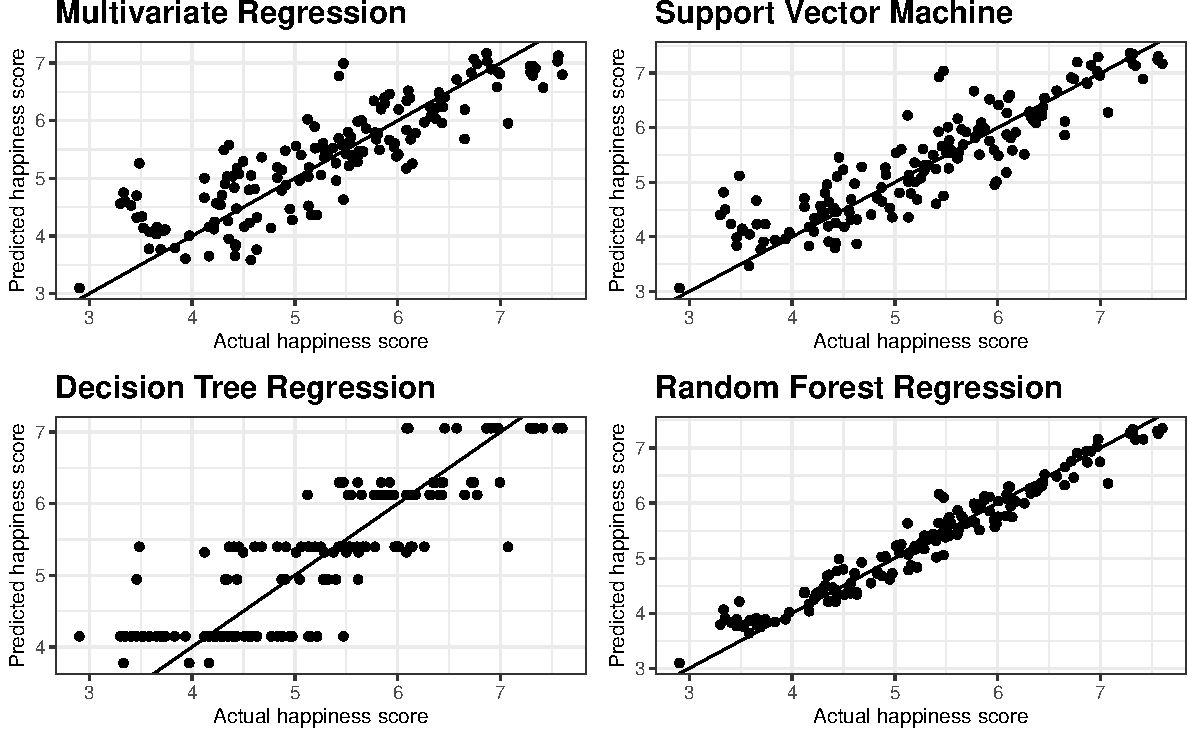
\includegraphics{Assignment4_files/figure-latex/training-1.pdf}
\caption{\label{fig:training}Model Training Split Ratio is 0.8}
\end{figure}

\hypertarget{random-forest-regression}{%
\subsubsection{Random Forest regression}\label{random-forest-regression}}

Random Forest Model have the variable selecting system (via bootstrapping) to decide the most significant tree and can reduce overwriting compared with decision tree.With that said, random forests are a strong modeling technique and much more robust comparing with many different methods \autocite{liberman2017}. We can see from the plot that this model have captured the data well in the past few years for various training set (see).

To get which are the most important variables we then check their loadings in RF model (see Table \ref{tab:varimp}).

\begin{table}

\caption{\label{tab:varimp}Variable importance for Random Forest model}
\centering
\begin{tabular}[t]{l|r}
\hline
  & IncNodePurity\\
\hline
\cellcolor{gray!6}{Economy} & \cellcolor{gray!6}{348.66900}\\
\hline
Health & 327.08463\\
\hline
\cellcolor{gray!6}{Freedom} & \cellcolor{gray!6}{169.32991}\\
\hline
Generosity & 97.79738\\
\hline
\end{tabular}
\end{table}

In the Table \ref{tab:varimp}, we conclude that the most important variables on explaining the happiness scores will be the Happiness and Health due to the loading for them are significant higher than others.

\newpage

\hypertarget{multivariate-linear-model-analysis.}{%
\subsection{Multivariate Linear Model Analysis.}\label{multivariate-linear-model-analysis.}}

One advantage of multivariate linear regression is that it can allow us to analyse the relationship between different variables in a statistical coherent way. For example, marginal effects and percentage changes.

In our classic linear model, which is

\[
\begin{aligned}
&\textbf{Classic Multivariate Linear Model}:\\
Happiness\ score=& Economy+Health+Generosity+Freedom
\end{aligned}
\]

We can see from Table \ref{tab:without}, in our classic linear model, they have similar loadings and all of them are significant, which we cannot tease out the important variables out of this model.

\begin{table}

\caption{\label{tab:without}Linear regression model for happiness scores without new data}
\centering
\begin{tabular}[t]{l|r|r|r|r}
\hline
  & Estimate & Std. Error & t value & Pr(>|t|)\\
\hline
\cellcolor{gray!6}{(Intercept)} & \cellcolor{gray!6}{2.437442} & \cellcolor{gray!6}{0.0752984} & \cellcolor{gray!6}{32.370444} & \cellcolor{gray!6}{0}\\
\hline
Health & 1.223204 & 0.1392052 & 8.787054 & 0\\
\hline
\cellcolor{gray!6}{Economy} & \cellcolor{gray!6}{1.454316} & \cellcolor{gray!6}{0.0841520} & \cellcolor{gray!6}{17.282015} & \cellcolor{gray!6}{0}\\
\hline
Freedom & 1.372180 & 0.1095802 & 12.522156 & 0\\
\hline
\cellcolor{gray!6}{Generosity} & \cellcolor{gray!6}{1.170207} & \cellcolor{gray!6}{0.1396671} & \cellcolor{gray!6}{8.378545} & \cellcolor{gray!6}{0}\\
\hline
\end{tabular}
\end{table}

In order to better analyse the relationships, I add two new variables, which are CPI values and the population size for each country. However, due to the limitation of the new dataset, we can only conduct our analysis based on the data up to 2020.

Moreover, due to the endogenous bias, the t-test here is biased so we cannot reject variables based on the p-value in this case.

\[
\begin{aligned}
log(score)= -4.6000-0.0008\ cpi+0.2591\ log(economy)\\-0.0026\ log(population)+0.0114\ log(health)+0.0032log(year)
\end{aligned}
\]

\begin{table}

\caption{\label{tab:unnamed-chunk-6}Multivariate Linear regression model for the log data}
\centering
\begin{tabular}[t]{l|r|r|r|r}
\hline
  & Estimate & Std. Error & t value & Pr(>|t|)\\
\hline
\cellcolor{gray!6}{(Intercept)} & \cellcolor{gray!6}{-4.5998547} & \cellcolor{gray!6}{11.5632413} & \cellcolor{gray!6}{-0.3977998} & \cellcolor{gray!6}{0.6909123}\\
\hline
cpi & -0.0007945 & 0.0001848 & -4.2993658 & 0.0000198\\
\hline
\cellcolor{gray!6}{log\_eco} & \cellcolor{gray!6}{0.2590779} & \cellcolor{gray!6}{0.0094044} & \cellcolor{gray!6}{27.5487182} & \cellcolor{gray!6}{0.0000000}\\
\hline
log\_population & -0.0025806 & 0.0036488 & -0.7072364 & 0.4796807\\
\hline
\cellcolor{gray!6}{log\_health} & \cellcolor{gray!6}{0.0113946} & \cellcolor{gray!6}{0.0041557} & \cellcolor{gray!6}{2.7419415} & \cellcolor{gray!6}{0.0062809}\\
\hline
year & 0.0031566 & 0.0057310 & 0.5507847 & 0.5819762\\
\hline
\end{tabular}
\end{table}

We can see that the total proportion of variance explained by the model with these variables are 60.49\%. For the 4 predictors, the economy status(GDP per capita) contribute most to the happiness scores than other variables.

\hypertarget{endogenity-and-sample-selection-bias-.}{%
\section{Endogenity and Sample Selection Bias .}\label{endogenity-and-sample-selection-bias-.}}

We only included 5 variables and total \(R^2\) is around 60.49\% in our model. Then, considering the happiness score can be affected by many prospects. There should have some latent variables that do affect the happiness score for example the education level and culture backgrounds. In other words, our model have an endogeneity issue, which we can solve it by either adding more related variables or use the two-stage least square model.

\begin{figure}
\centering
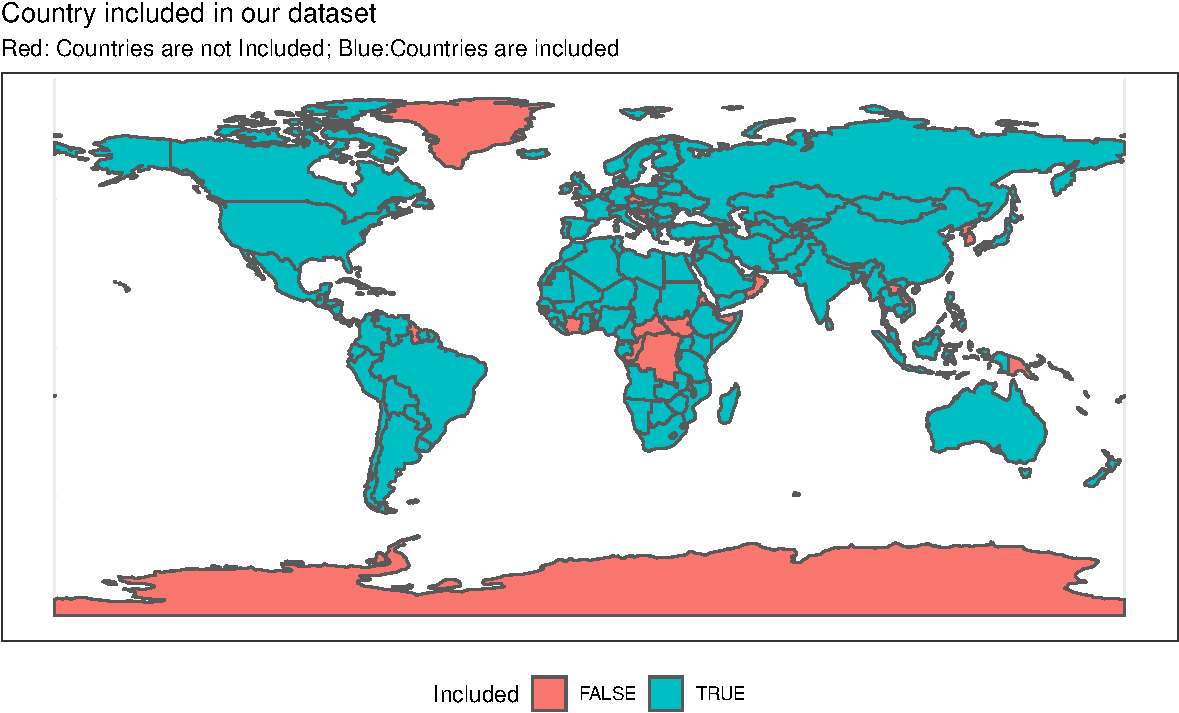
\includegraphics{Assignment4_files/figure-latex/worldmapall-1.pdf}
\caption{\label{fig:worldmapall}Colour the country that have included in Worldmap}
\end{figure}

Apparently, our model have some bias in selecting our sample. In our report, there are 34 are not included, which have been colored in red from Figure \ref{fig:worldmapall}. In our sample, we can see countries are not included either from sparsely populated area or developing countries, which indicates that our sample is not random enough and exists a sample selection bias. To solve this, sample selection models such as Heckman model or Tobit can be considered in Econometrics areas.

\newpage

\hypertarget{potential-problems}{%
\section{Potential Problems}\label{potential-problems}}

The diagnostic of our regression model is shown in Figure \ref{fig:resd}. From the Residual and Fitted plot, we can see it has non-constant variance across the fitted value, which means the presence of Hetroskedasticity. Moreover,both the error distribution (see Figure \ref{fig:density}) and the Q-Q plot Figure (see Figure \ref{fig:qq} also suggest the density of our model is close to a normal distribution but seems there are some influences by outliers. In the

\begin{figure}
\centering
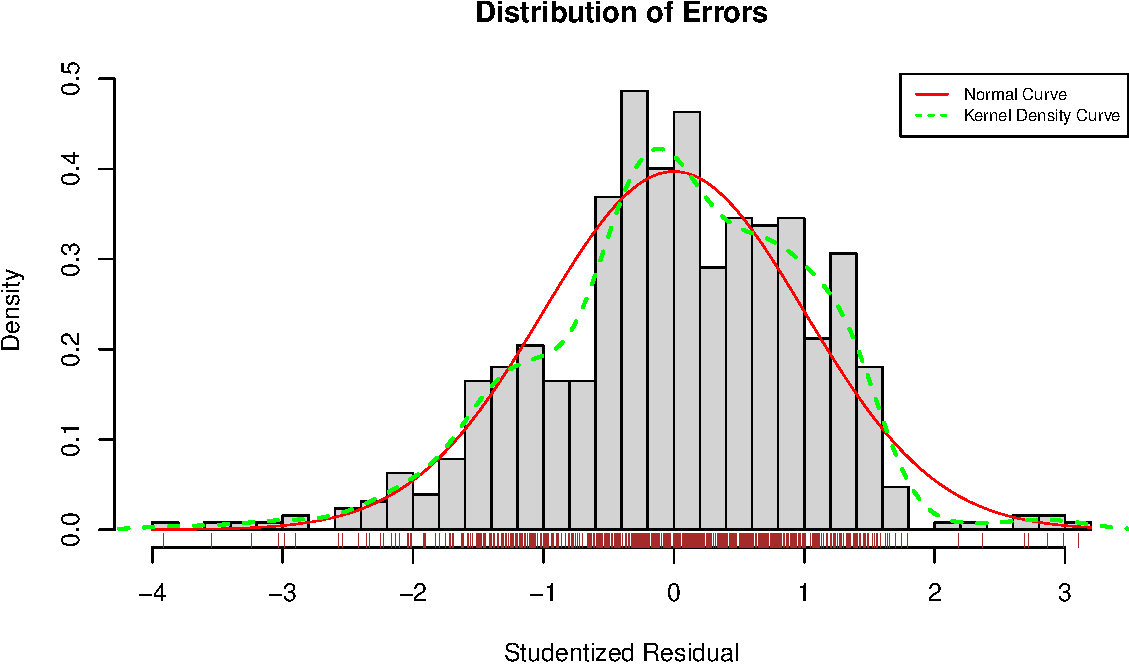
\includegraphics{Assignment4_files/figure-latex/density-1.pdf}
\caption{\label{fig:density}Distribution of the residual term}
\end{figure}

\begin{figure}
\centering
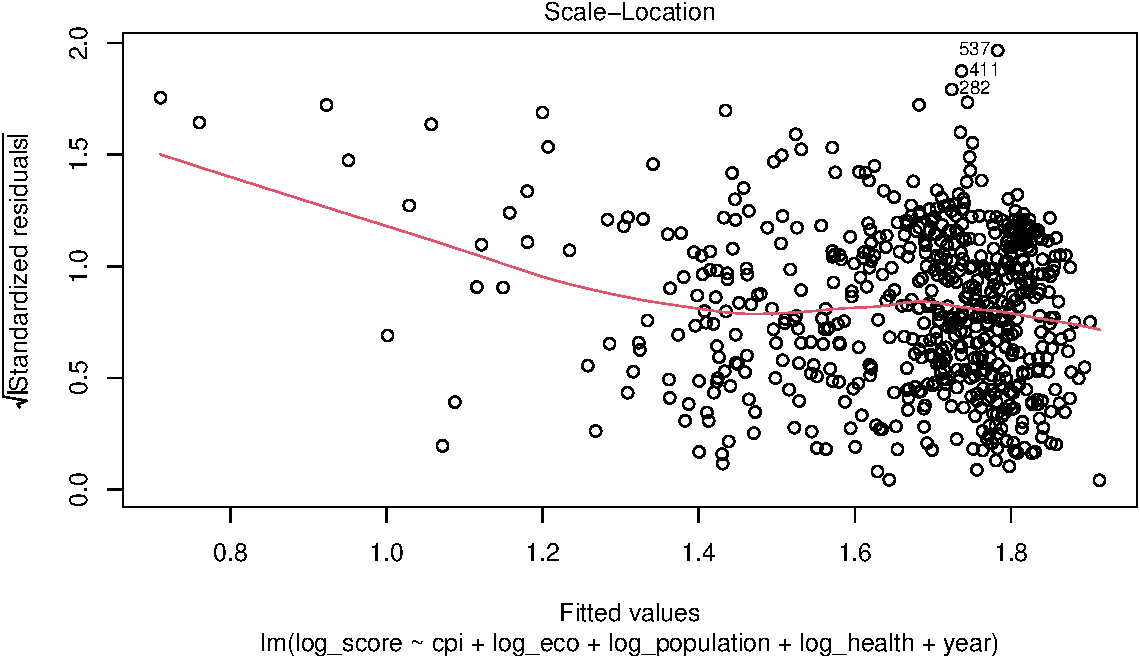
\includegraphics{Assignment4_files/figure-latex/resd-1.pdf}
\caption{\label{fig:resd}Residual vs Fitted value plot (with standardised residuals)}
\end{figure}

\begin{figure}
\centering
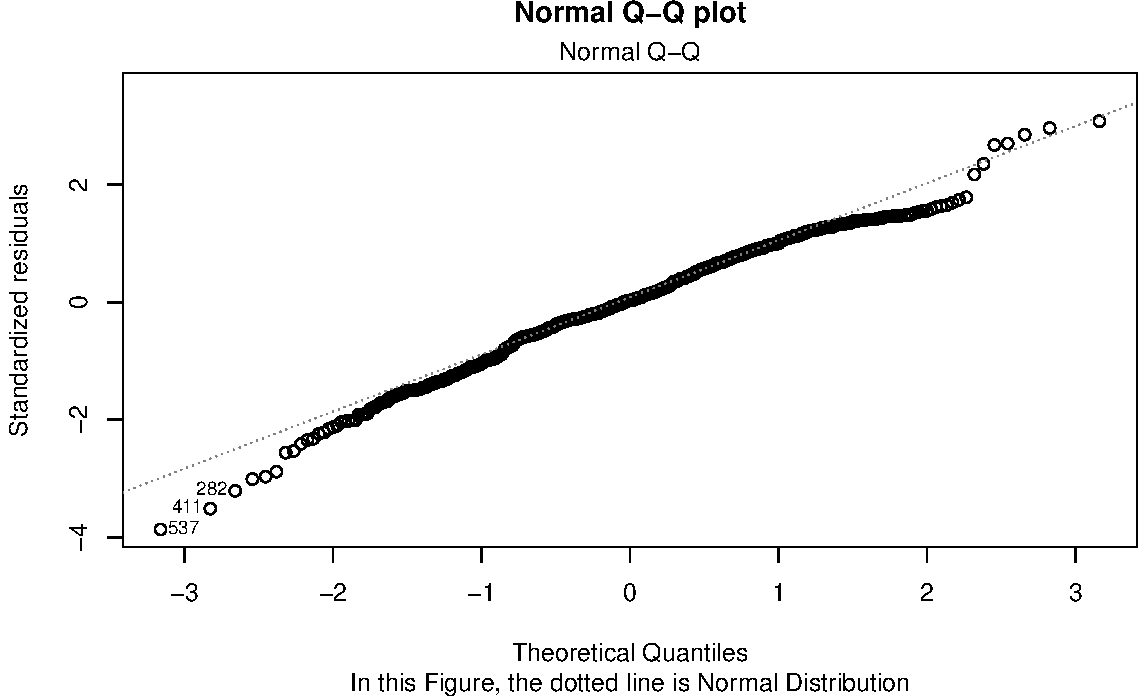
\includegraphics{Assignment4_files/figure-latex/qq-1.pdf}
\caption{\label{fig:qq}Q-Q plot fitted model residual density vs normal distribution residual density}
\end{figure}

\begin{figure}
\centering
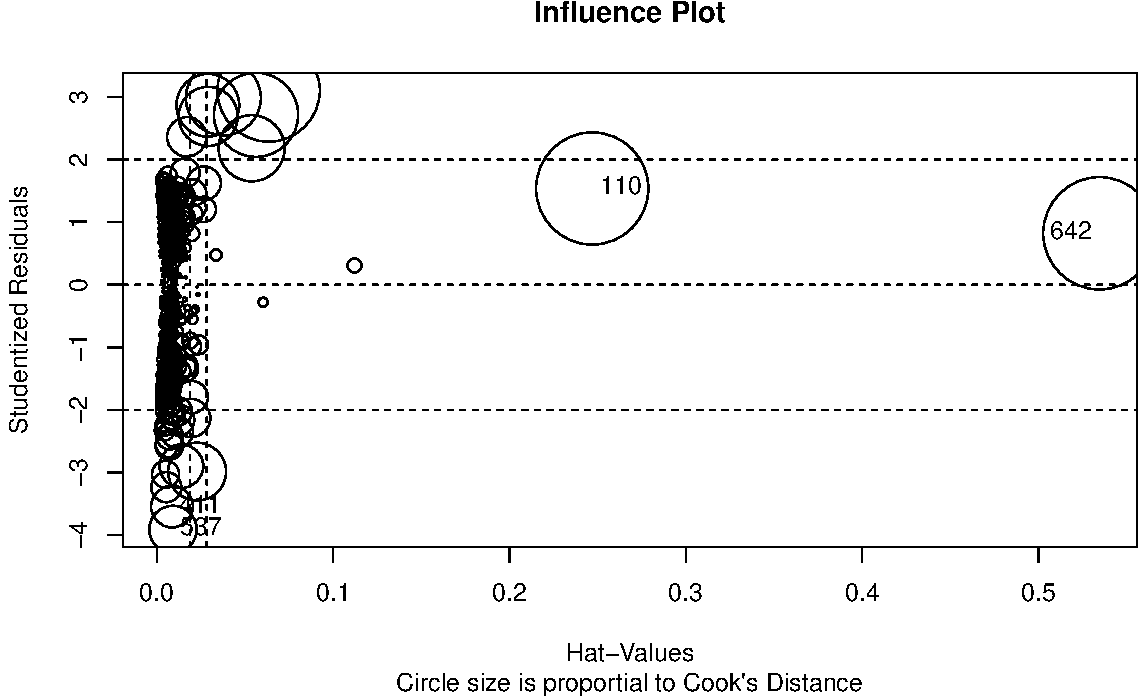
\includegraphics{Assignment4_files/figure-latex/inf-1.pdf}
\caption{\label{fig:inf}Influence Plot, the bigger circle means outliers}
\end{figure}

\clearpage

\hypertarget{concclusion}{%
\section{Concclusion}\label{concclusion}}

\clearpage

\printbibliography[title=Appendix]

\end{document}
